\documentclass[10pt,usenames,dvipsnames,svgnames,table]{beamer}
\usetheme{Warsaw}

\usepackage[english]{babel}
\usepackage[latin1]{inputenc}
\usepackage{amssymb}
\usepackage{graphicx}
\usepackage{epstopdf}
\graphicspath{ {./images/} }
\allowdisplaybreaks
\usepackage{tikz}
\setbeamertemplate{bibliography item}[text] %remove the icon
\setbeamertemplate{frametitle continuation}{}

\title{Optimal Location of Car Wreck Adjusters}
\subtitle{IV Congreso Nacional SMIO}
\author[Luis Maltos, Roger R\'ios, Angelica Salazar, M. Gpe. Villarreal]{
  L. A. Maltos-Ortega \inst{1},
  R. Z. R\'ios-Mercado \inst{1},
  M. A. Salazar-Aguilar \inst{1}
  \and M. G. Villareal Marroquin \inst{2}}

\institute[PISIS]{
  \inst{1} Posgrado en Ingenier\'ia de Sistemas \\
  FIME / UANL \and
  \inst{2} CIMAT Unidad Monterrey
}

\date[Oct 2015]{October 2015}

\AtBeginSubsection{
  \frame{\frametitle{Table of Contents}
    \tableofcontents[currentsubsection]}
}

\begin{document}
\begin{frame}
  \titlepage
\end{frame}

\begin{frame}{Contents}
  \tableofcontents
\end{frame}

%%% Introduction %%%

%En ella se deben exponer brevemente pero con absoluta claridad, 
% la novedad y actualidad del tema,
% el objeto de la investigación,
% sus objetivos,
% la hipótesis de trabajo,
% el fundamento metodológico y
% los métodos utilizados para realizar el trabajo de investigación.
%Es decir, que la introducción es la fundamentación científica de la tesis en forma resumida.

\section{Introduction}
\begin{frame}

  The aim of this work is to support decision making regarding
  the location and redeployment of insurance agents to attend car wrecks.

  The idea is to develop models and methods for 
  (a) improving the service offered by insurance agents, 
  helping them arrive to the accident sites sooner, and 
  (b)  determining the number of adjusters required to perform 
  the service within the desired standards.

\end{frame}

\subsection{Problem}
\frame{
  \textit{The main goal is to determine the optimal bases (locations) 
    for placing the insurance company adjusters, 
    so as to minimize the average or maximum response time
    from customer calls when accidents occur.}
  \begin{center}
    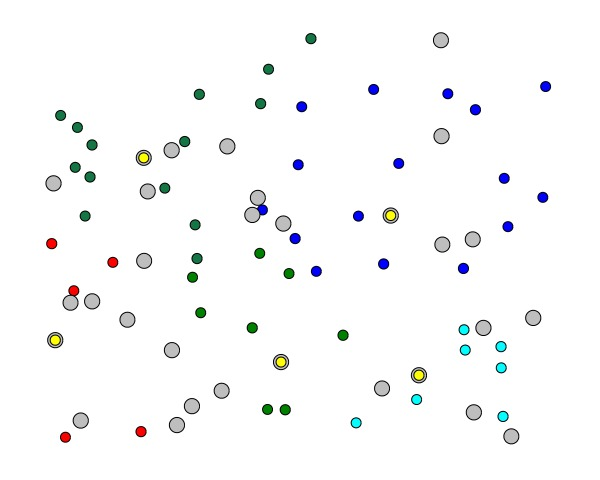
\includegraphics[scale=0.40]{graph_problem}
  \end{center}
}

\subsection{Motivation}
\begin{frame}
  When a car accident occurs, traffic congestion starts to pile up.
  This is because customers are not allowed to move their vehicles
  until the adjuster arrives.  
  The adjuster must record and determine the causes of the accident, 
  in order to move the car from the accident area and restore the flow.
  \begin{center}
    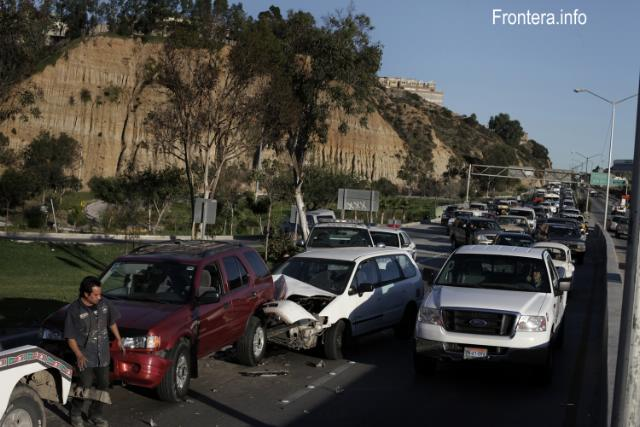
\includegraphics[scale=0.25]{389200-G}
  \end{center}
\end{frame}

\subsection{Background}
\begin{frame}[allowframebreaks]
  Richard Larson (1974) \cite{larson1974hypercube,larson1975approximating}
  proposes the Hypercube, and A-Hypercube models
  for a queuing approach for locating multiple facilities.

  James P. Jarvis (1985) \cite{jarvis1985approximating} incorporates
  location dependent service times characteristics for the A-Hypercube model,
  developing an approximation model for a spatially distributed queuing system
  under general service time assumptions.

  Berman et al. (1987) \cite{berman1987stochastic}
  formulate the Stochastic Queue p-Median problem (SQpM),
  and propose a heuristic approach for locating cooperative service facilities
  on a network.

  Goldberg et al. (1990) \cite{goldberg1990validating}
  propose a nonlinear integer programming model
  based on general service time approximation
  for spatially distributed queuing systems.

\end{frame}

\subsection{Hypercube queueing model}
\begin{frame}
Solution procedures for probabilistic models that use the hypercube model
with optimization procedures 
for server deployment can be found in the literature, for example
Larson (1979) \cite{larson1978structural}, 
Berman et al. (1985,1987) \cite{berman1985optimal,berman1987stochastic}, 
Saydam and Aytug (2003) \cite{saydam2003accurate}, 
Rajagopalan et al. (2008) \cite{rajagopalan2008multiperiod} and 
Iannoni et al. (2008a, 2008b) \cite{iannoni2008hypercube,iannoni2009optimization},
\end{frame}

%%% Models %%%
% Validating and applying a model for locating emergency medical vehicles in Tucson, AZ
% Goldberg 1990

\section{Models}
\subsection{Model A}

\begin{frame}
  This model is based on Goldberg's model, and it contains assignment
  variables for all possible orders.

  The following assumptions are considered in the model:
  \begin{itemize}
  \item The probability that an adjuster is busy is $\rho$
    and is unaffected by the state of the system
  \item There is a strict ordering of the bases preferred for each zone
    that does not depend on the current state of the system
  \item All calls are answered by an adjuster originating from its base,
    not en route back to the base
  \item The arrival of calls to the system follows a stationary distribution
  \item The model is presented using a 0-queue assumption.
  \end{itemize}
  
\end{frame}


\begin{frame}
  Parameters:
  \begin{itemize}
  \item $V$ set of demand points, with $|V| = n$
  \item $W$ set of potential site for adjusters/facilities, with $|W| = m$
  \item $p$ number of available adjusters
  \item $K$  set of possible orders $\{1,2\ldots,p\}$
  \item $\rho$ is the utilization of each vehicle
  \item $t_{ij}$ is the expected travel time between zone \textit{i} and base \textit{j}.
  \item $h_{ij}^{k}$ is the probability that $j$ serves customer $i$ given that
    is the $k$-th preferred.
  \item $S_{ij} = \{r\in W | t_{ir} < t_{ij}\}$
  \end{itemize}
  
  Variables:
  \begin{itemize}
  \item $x_j =
    \begin{cases} 
      1 & \mbox{if an adjuster is at node } j \\
      0 & \mbox{otherwise}
    \end{cases}$
  \item $y_{ij}^k =
    \begin{cases} 
      1 & \mbox{if adjuster in } j \mbox{, is the k-th to cover customer }i \\
      0 & \mbox{otherwise}
  \end{cases}$
  \end{itemize}
\end{frame}

\begin{frame}[allowframebreaks]{}{}

{\small
  \begin{equation}
    \min \, \sum_{j=1}^{m}{\sum_{\ell=1}^{k}{\sum_{i=1}^{n}{h_{ij}^{\ell}t_{ij}y_{ij}^{\ell}}}}
  \end{equation}
}
{\small
  \begin{align}
    \sum_{j \in W}{x_j} & = p               &                                  &\\
    \sum_{j \in W}{y_{ij}^{k}} & = 1        &          i \in V, k &\in K \\
    y_{ij}^{k} & \leq x_j                   &  i \in V,j \in W, k &\in K \\
    \sum_{k = 1}^{p}{y_{ij}^{k}} & \leq x_j &          i \in V, j &\in W \\
    y_{ij}^{k} &\leq \sum_{r\in S_{ij}}{y_{ir}^{k-1}} &  i \in V,j \in W, k &\in K/\{1\} \\
    x_{j} & \in \{0,1\}      &                  j &\in W \nonumber\\
    y_{ij}^{k} & \in \{0,1\} &  i \in V,j \in W,k &\in K \nonumber
  \end{align}
}
\end{frame}

\begin{frame}
  This model was tested with a benchmark instance of 30 points, 
  which sets $V$ and $W$ are the same.
  For values of $p = 1,\ldots,7$ the optimal solution was found in less than one minute.

  For other benchmark instances was impossible to find the solution
  because they have more than 300 points, and the proposed model grows to over one million variables.
%  For some large instances ($n = 50$ , $m = 30$)%
\end{frame}

% A model for the Stochastic Queue p-Median Problem
% Created by Luis Maltos & Roger Rios
% 2015

\subsection{Model B}
  
\begin{frame}
  This model was developed with the idea that is unlikely that
  the farthest adjusters serve customers on cases where the system does not become congested.
  In these cases we can make the assumption that the probability of being served by the $\ell$-th 
  adjuster is almost zero, where $\ell$ is large enough but less than $p$.

  Parameters:
  \begin{itemize}
  \item $M$ is a large integer
  \item $\ell$ the number of allowed adjusters per customer
  \item $a_{ik}$ the $k$-th preferred location server regarding the customer $i$.
  \end{itemize}

  Variables:
  \begin{itemize}
  \item $z_j$ the number of adjusters placed at site $j$
  \item $y_{ij}^k$ if facility $j$, is the $k$-th to cover customer $i$
  \end{itemize}

\end{frame}

\begin{frame}[allowframebreaks]
  The objective, and the constraints (2)-(5) 
  are practically the same as in model A,
  with the difference that binary variables $x_j$ from Model A
  are replaced by integer variables $z_j$ inspired by the results of Berman,
  and the addition of the following binary variables
  {\scriptsize
    \begin{itemize}
    \item $u_{ij} = \begin{cases} 1 & \mbox{if the number of adjusters between } i \mbox{ and } j \mbox{, inclusive, is less than } \ell \\
      0 & \mbox{otherwise}
    \end{cases}$
    \item $v_{ij} = \begin{cases} 1 & \mbox{if the number of adjusters between } i \mbox{ and } j \mbox{, is less than } \ell - 1 \\
      0 & \mbox{otherwise}
    \end{cases}$
    \end{itemize}
  }

{\footnotesize
  \begin{align}
    \sum_{r = 1}^{k \mid a_{ik}=j}{z_{a_{ir}}} + (p-\ell) u_{ij} & \leq p &  i \in V, j &\in W \\
    \sum_{r = 1}^{k \mid a_{ik}=j}{z_{a_{ir}}} + M u_{ij} & \geq \ell+1   &  i \in V, j &\in W \\
    \sum_{k = 1}^{\ell}{y_{ij}^{k}} + M (1 - u_{ij}) & \geq z_j           &  i \in V, j &\in W
  \end{align}
  
  \begin{align}
    \sum_{r = 1}^{k \mid a_{i(k+1)}=j}{z_{a_{ir}}} + (p-(\ell-1)) v_{ij} & \leq p                                     &  i \in V, j &\in W\\
    \sum_{r = 1}^{k \mid a_{i(k+1)}=j}{z_{a_{ir}}} + M v_{ij}         & \geq \ell                                     &  i \in V, j &\in W\\
    \sum_{k=1}^{k}{y_{ij}^{k}} + M (1 - v_{ij} + u_{ij}) & \geq \ell - \sum_{r = 1}^{k \mid a_{i(k+1)}=j}{z_{a_{ir}}} &  i \in V, j &\in W\\
    \sum_{k=1}^{k}{y_{ij}^{k}} - M (1 - v_{ij} + u_{ij}) & \leq \ell - \sum_{r = 1}^{k \mid a_{i(k+1)}=j}{z_{a_{ir}}} &  i \in V, j &\in W\\
    y_{ij}^{k} & \leq u_{ij} + v_{ij}  &        i \in V,j &\in W \\
    z_j & \in \{0,1,\ldots,p\}         &                j &\in V \nonumber\\
    y_{ij}^{k} & \in \{0,1\}           &  i\in V,j\in W,k &\in I \nonumber\\
    u_{ij},v_{ij} & \in \{0,1\}        &        i \in V,j &\in W \nonumber
  \end{align}
}
\end{frame}

%%% Results %%%

\section{Results}
\subsection{Experimentation}
\begin{frame}
  All experiments were evaluated in a Lanix Spine BW
  Processor Intel Xenon, CPU E5-2867W, 3.10 GHz.
  With operative system Ubuntu 14.04.3 LTS
  The models were solved with CPLEX 12.6.0.0,
  and they were coded in C++.
\end{frame}

\begin{frame}
  Different random instances were generated
  to validate the proposed formulations.
  For $n = 100$ we created 3 instances with $m = 20,30,40$,
  and different values of $p$, shown in the following table.
  \begin{table}
    \centerign
    \begin{tabular}{|c|c|c|}\hline
      n & m & p \\ \hline
      100 & 20 & 5-18 \\
      100 & 30 & 7-25 \\
      100 & 40 & 9,10 \\
      \hline
    \end{tabular}
  \end{table}
  
  The Model A was solved to optimality for all the values of $p$ when $m = 20$,
  for the rest of the values of $m$, none optimal solution was reported in less than one hour.

  The Model B was tested with each combination of $n,m,p$ and $\ell$ from $1,\ldots,p$.

\end{frame}

\begin{frame}{Model B}
  Relation of $\frac{\ell}{p}$ versus the solution time.
  \begin{center}
    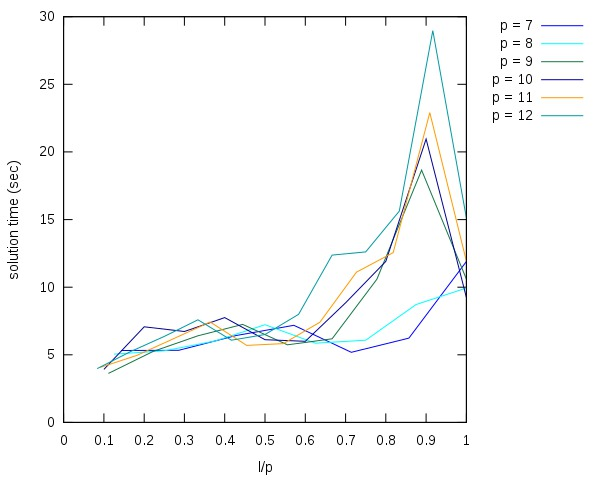
\includegraphics[scale=0.25]{grafica_01}
    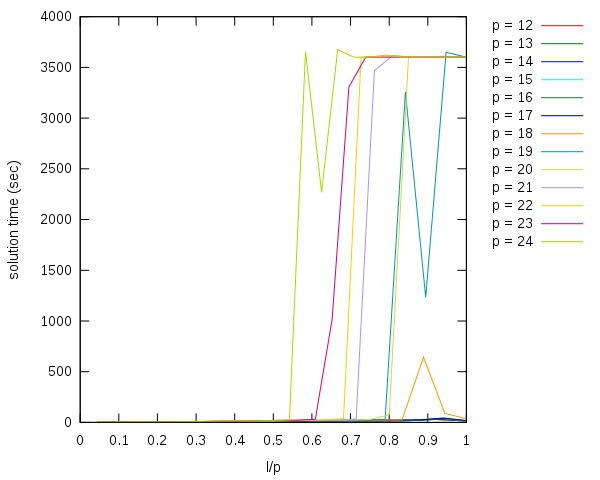
\includegraphics[scale=0.25]{grafica_02}
  \end{center}
\end{frame}

\begin{frame}{Model B}

  The solution times increase drastically as $\ell$ approximates to $p$
  
  \begin{center}
    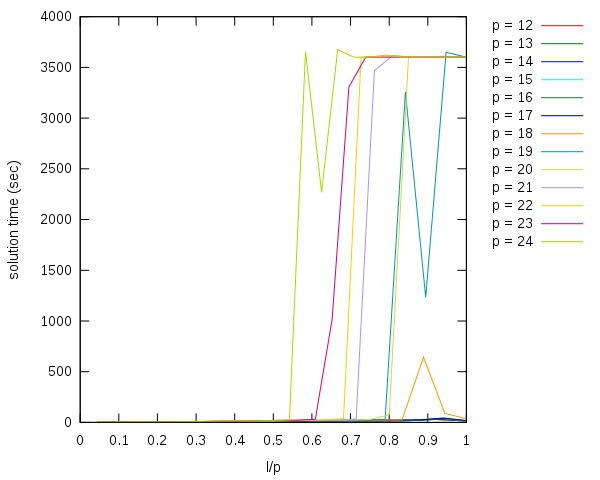
\includegraphics[scale=0.25]{grafica_02}
    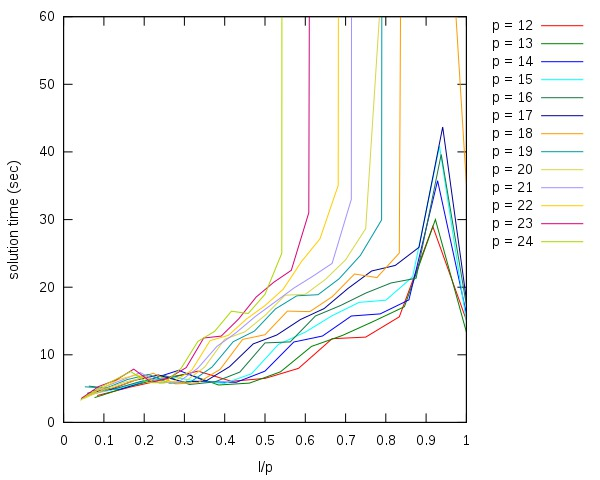
\includegraphics[scale=0.25]{grafica_03}
  \end{center}
  
\end{frame}

\begin{frame}{Model B}

  For medium values of $p$, the value of the objective function does not change
  for medium/small to large values of $\ell$, where the optimal solution is obtained.

  \begin{center}
    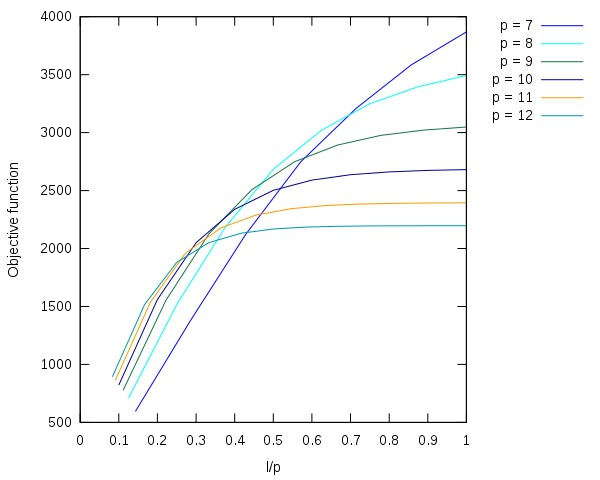
\includegraphics[scale=0.25]{grafica_04}
    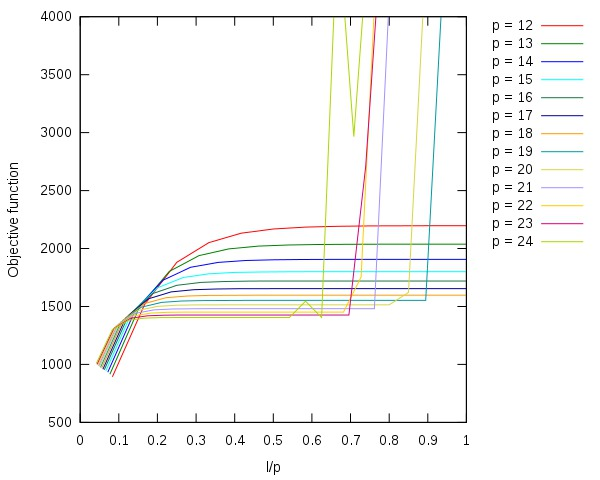
\includegraphics[scale=0.25]{grafica_05}
  \end{center}
  
\end{frame}

%% Caso 100 30 12
\frame{\begin{figure}[h!]\centering{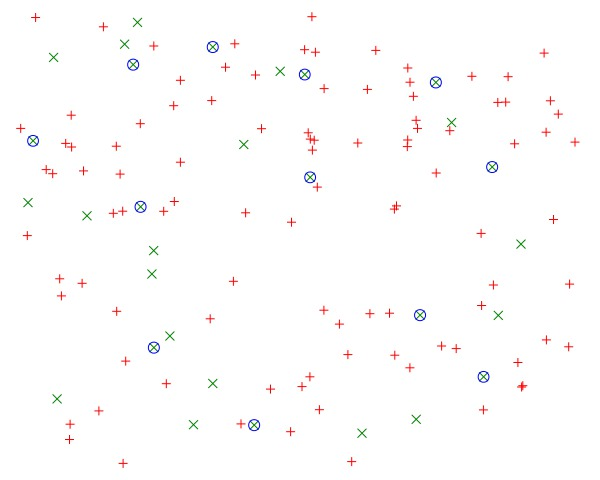
\includegraphics[scale=0.35]{Test_100_30_12_01}\caption{n = 100, m = 30, p = 12, l = 1}}\end{figure}}
\frame{\begin{figure}[h!]\centering{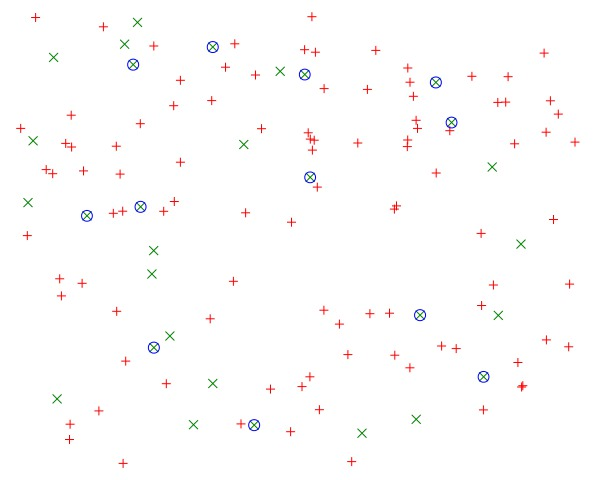
\includegraphics[scale=0.35]{Test_100_30_12_02}\caption{n = 100, m = 30, p = 12, l = 2}}\end{figure}}
\frame{\begin{figure}[h!]\centering{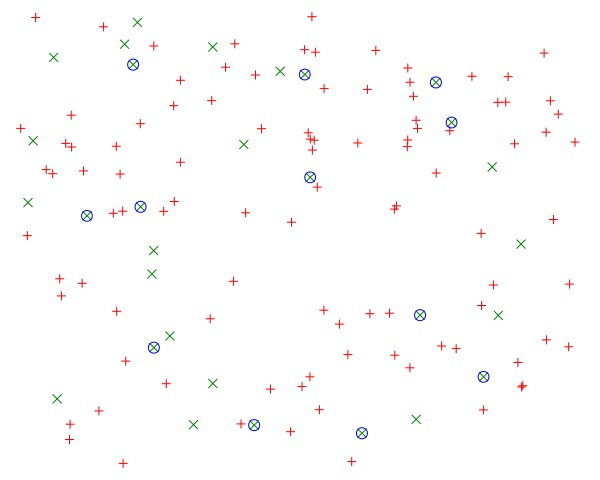
\includegraphics[scale=0.35]{Test_100_30_12_03}\caption{n = 100, m = 30, p = 12, l = 3}}\end{figure}}
\frame{\begin{figure}[h!]\centering{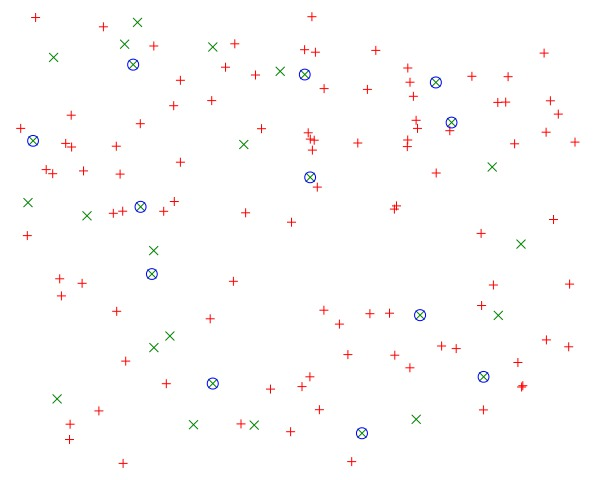
\includegraphics[scale=0.35]{Test_100_30_12_04}\caption{n = 100, m = 30, p = 12, l = 4}}\end{figure}}
\frame{\begin{figure}[h!]\centering{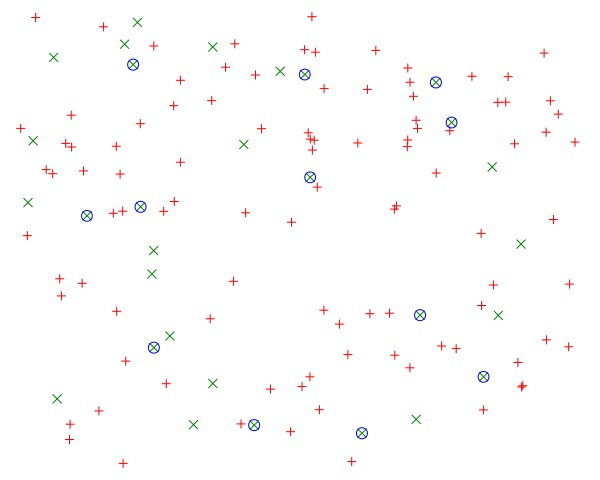
\includegraphics[scale=0.35]{Test_100_30_12_05}\caption{n = 100, m = 30, p = 12, l = 5}}\end{figure}}
\frame{\begin{figure}[h!]\centering{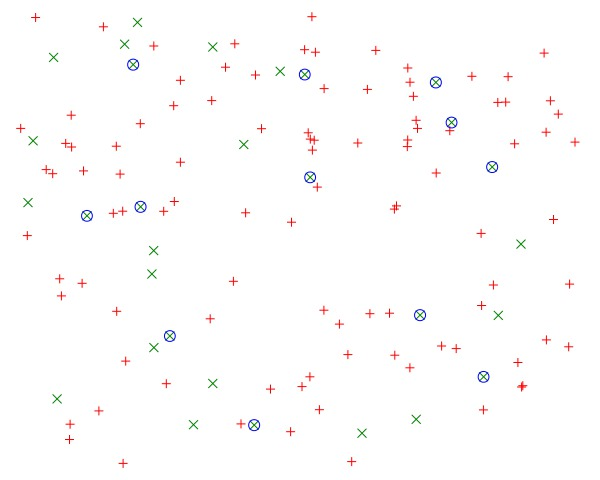
\includegraphics[scale=0.35]{Test_100_30_12_06}\caption{n = 100, m = 30, p = 12, l = 6}}\end{figure}}
\frame{\begin{figure}[h!]\centering{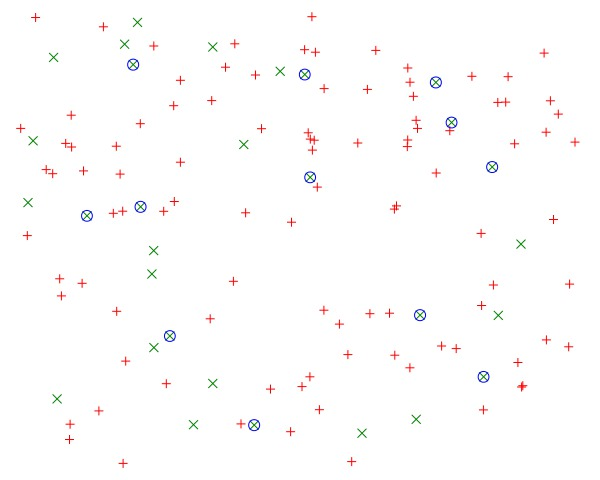
\includegraphics[scale=0.35]{Test_100_30_12_07}\caption{n = 100, m = 30, p = 12, l = 7}}\end{figure}}
\frame{\begin{figure}[h!]\centering{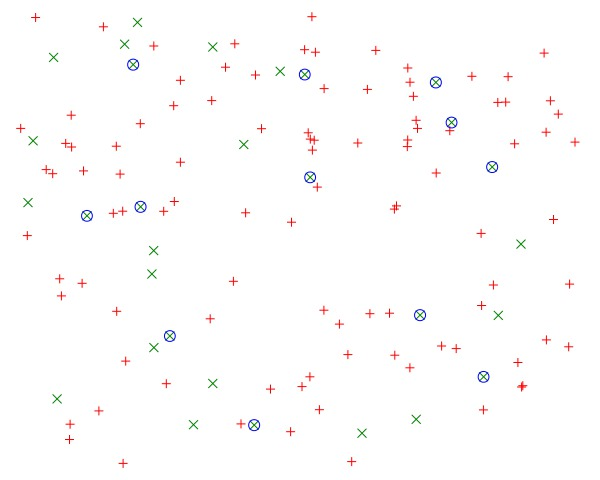
\includegraphics[scale=0.35]{Test_100_30_12_08}\caption{n = 100, m = 30, p = 12, l = 8}}\end{figure}}
\frame{\begin{figure}[h!]\centering{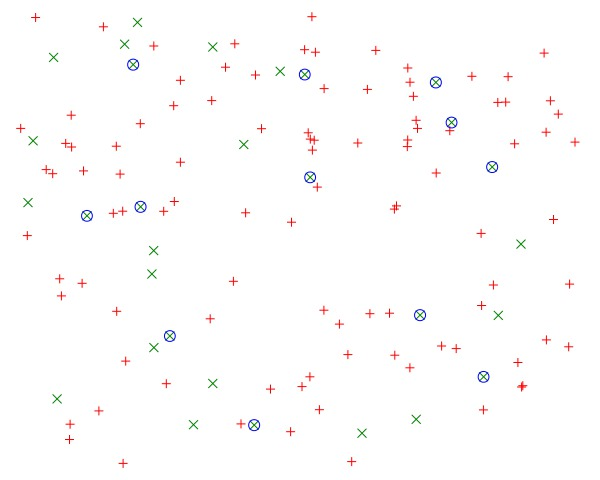
\includegraphics[scale=0.35]{Test_100_30_12_09}\caption{n = 100, m = 30, p = 12, l = 9}}\end{figure}}
\frame{\begin{figure}[h!]\centering{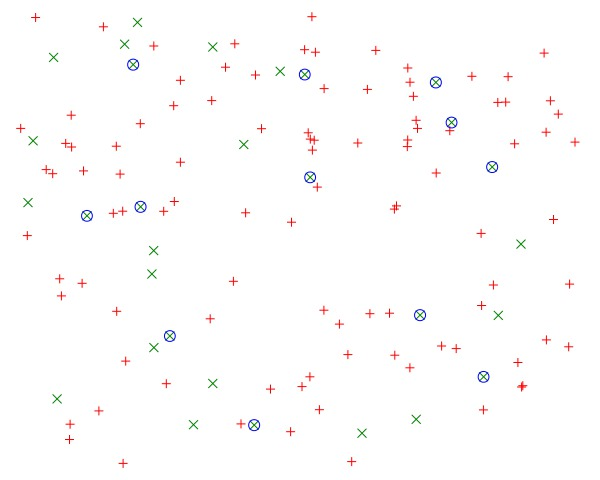
\includegraphics[scale=0.35]{Test_100_30_12_10}\caption{n = 100, m = 30, p = 12, l = 10}}\end{figure}}
\frame{\begin{figure}[h!]\centering{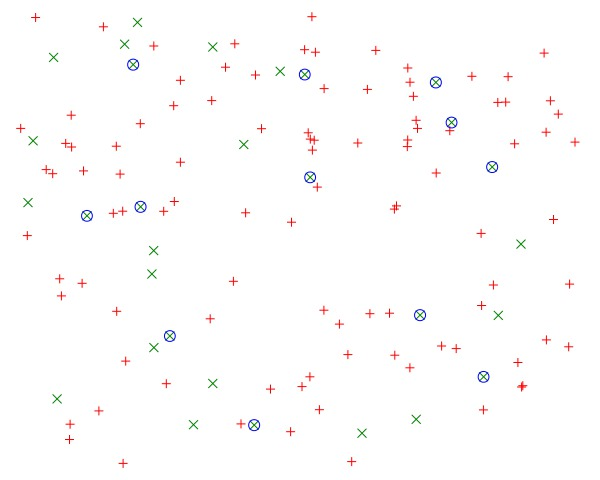
\includegraphics[scale=0.35]{Test_100_30_12_11}\caption{n = 100, m = 30, p = 12, l = 11}}\end{figure}}
\frame{\begin{figure}[h!]\centering{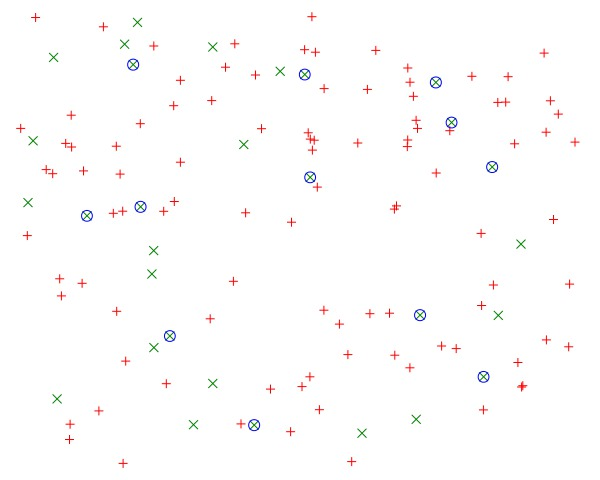
\includegraphics[scale=0.35]{Test_100_30_12_12}\caption{n = 100, m = 30, p = 12, l = 12}}\end{figure}}

\frame{\begin{figure}[h!]\centering{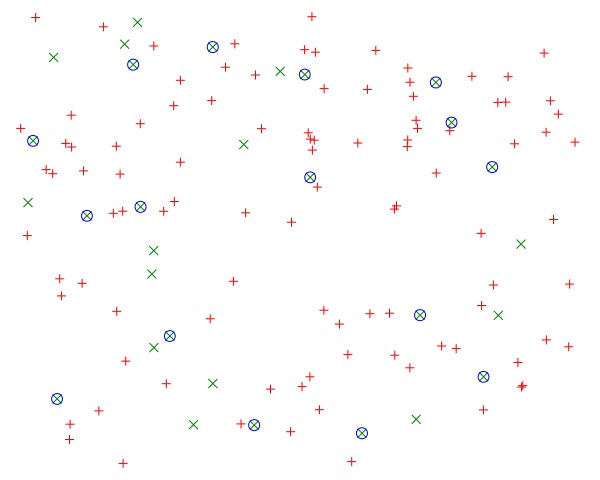
\includegraphics[scale=0.35]{Test_100_30_16_01}\caption{n = 100, m = 30, p = 16, l = 1}}\end{figure}}
\frame{\begin{figure}[h!]\centering{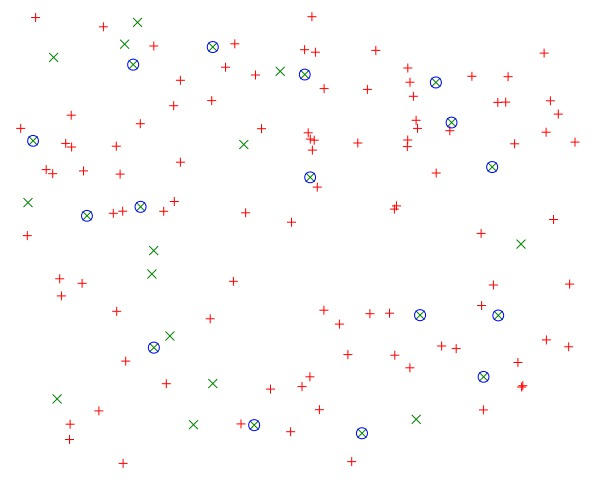
\includegraphics[scale=0.35]{Test_100_30_16_02}\caption{n = 100, m = 30, p = 16, l = 2}}\end{figure}}
\frame{\begin{figure}[h!]\centering{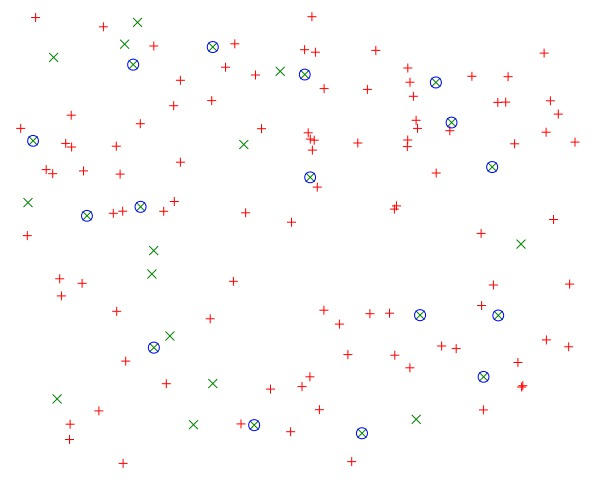
\includegraphics[scale=0.35]{Test_100_30_16_03}\caption{n = 100, m = 30, p = 16, l = 3}}\end{figure}}
\frame{\begin{figure}[h!]\centering{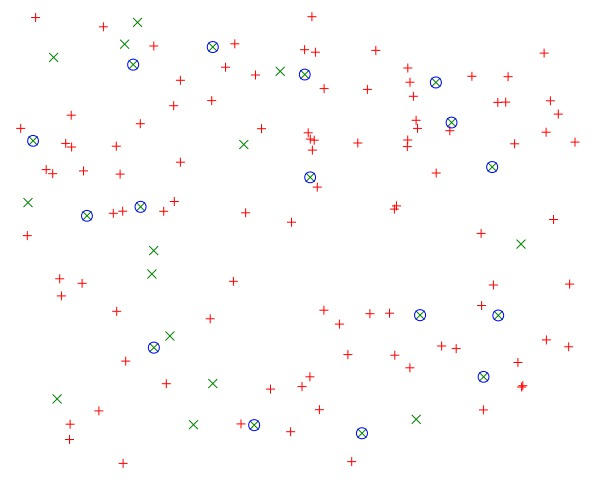
\includegraphics[scale=0.35]{Test_100_30_16_04}\caption{n = 100, m = 30, p = 16, l = 4}}\end{figure}}
\frame{\begin{figure}[h!]\centering{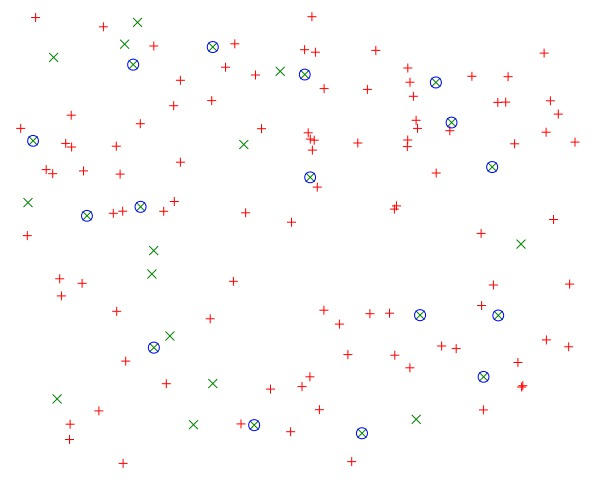
\includegraphics[scale=0.35]{Test_100_30_16_05}\caption{n = 100, m = 30, p = 16, l = 5}}\end{figure}}
\frame{\begin{figure}[h!]\centering{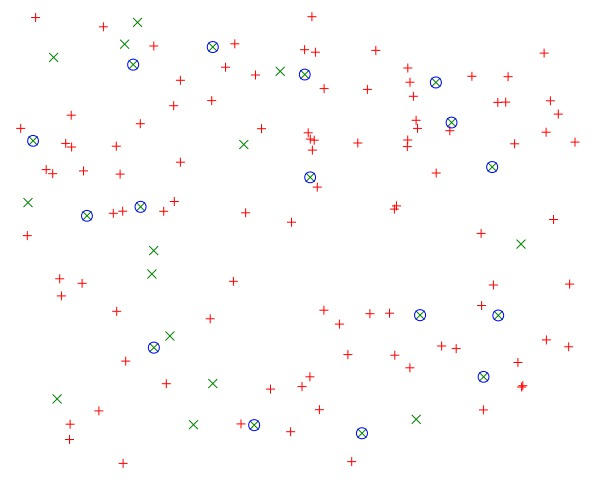
\includegraphics[scale=0.35]{Test_100_30_16_06}\caption{n = 100, m = 30, p = 16, l = 6}}\end{figure}}
\frame{\begin{figure}[h!]\centering{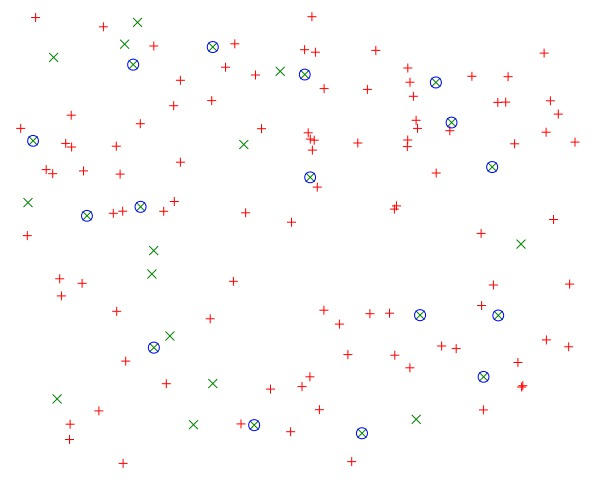
\includegraphics[scale=0.35]{Test_100_30_16_07}\caption{n = 100, m = 30, p = 16, l = 7}}\end{figure}}
\frame{\begin{figure}[h!]\centering{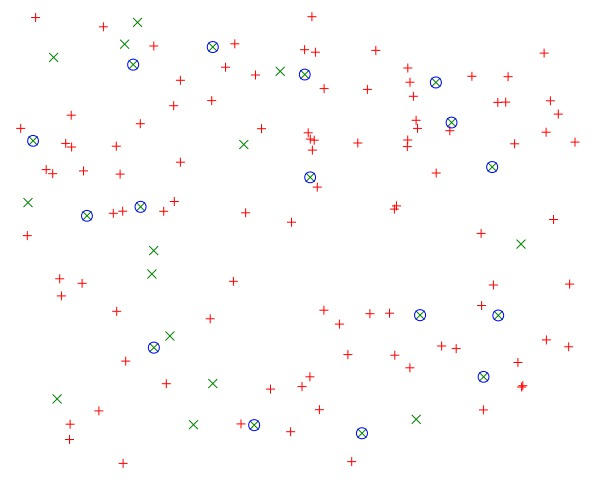
\includegraphics[scale=0.35]{Test_100_30_16_08}\caption{n = 100, m = 30, p = 16, l = 8}}\end{figure}}
\frame{\begin{figure}[h!]\centering{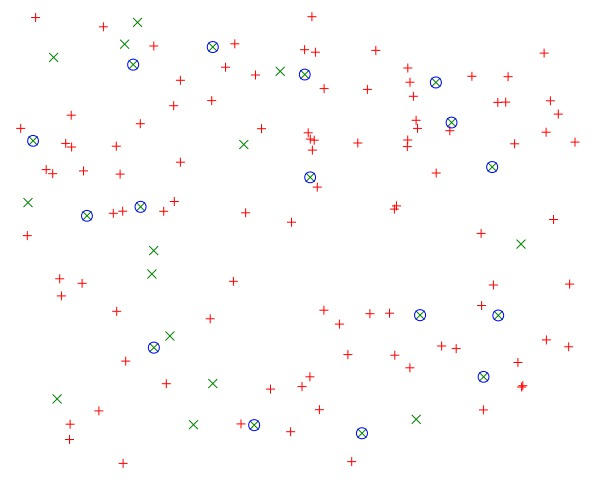
\includegraphics[scale=0.35]{Test_100_30_16_09}\caption{n = 100, m = 30, p = 16, l = 9}}\end{figure}}
\frame{\begin{figure}[h!]\centering{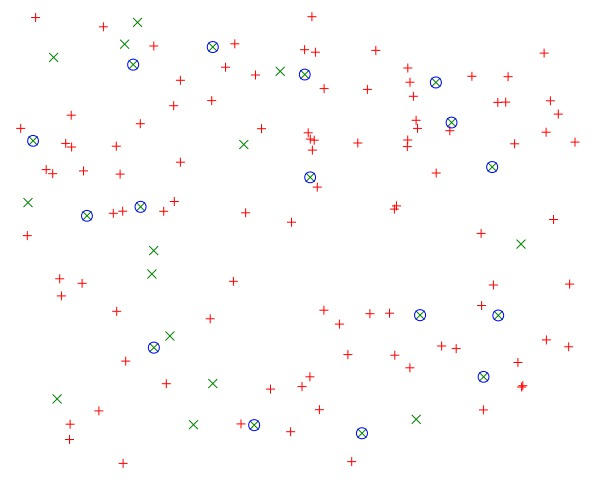
\includegraphics[scale=0.35]{Test_100_30_16_10}\caption{n = 100, m = 30, p = 16, l = 10}}\end{figure}}
\frame{\begin{figure}[h!]\centering{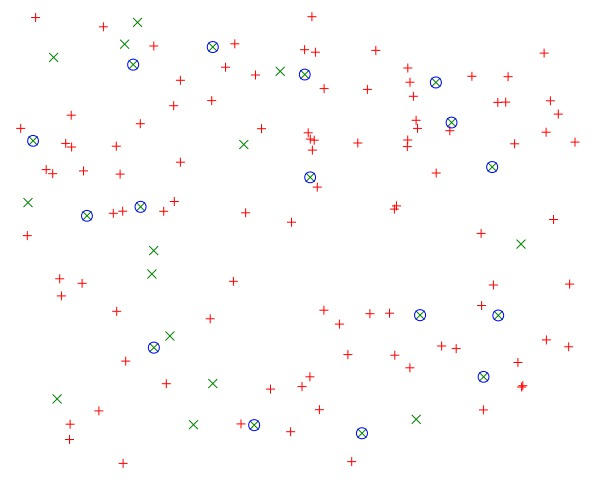
\includegraphics[scale=0.35]{Test_100_30_16_11}\caption{n = 100, m = 30, p = 16, l = 11}}\end{figure}}
\frame{\begin{figure}[h!]\centering{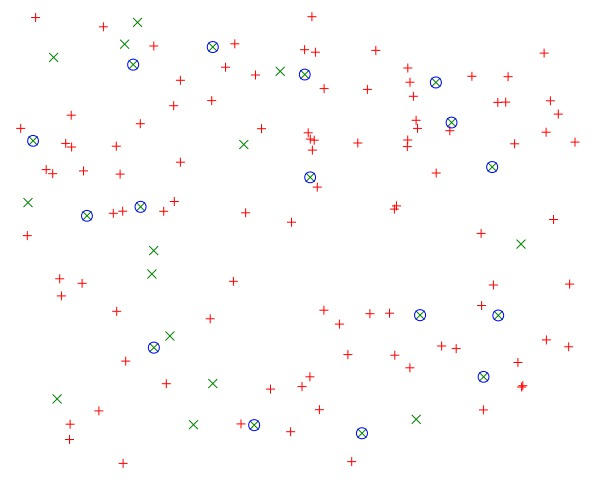
\includegraphics[scale=0.35]{Test_100_30_16_12}\caption{n = 100, m = 30, p = 16, l = 12}}\end{figure}}
\frame{\begin{figure}[h!]\centering{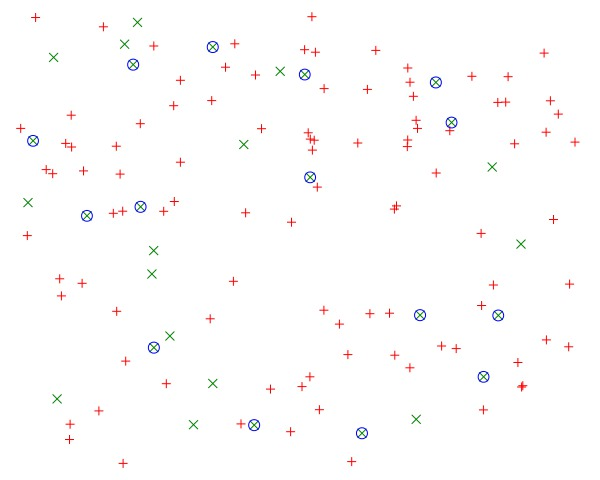
\includegraphics[scale=0.35]{Test_100_30_16_13}\caption{n = 100, m = 30, p = 16, l = 13}}\end{figure}}
\frame{\begin{figure}[h!]\centering{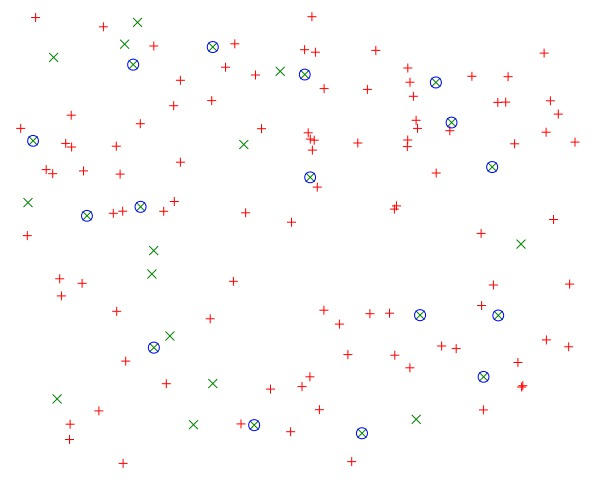
\includegraphics[scale=0.35]{Test_100_30_16_14}\caption{n = 100, m = 30, p = 16, l = 14}}\end{figure}}
\frame{\begin{figure}[h!]\centering{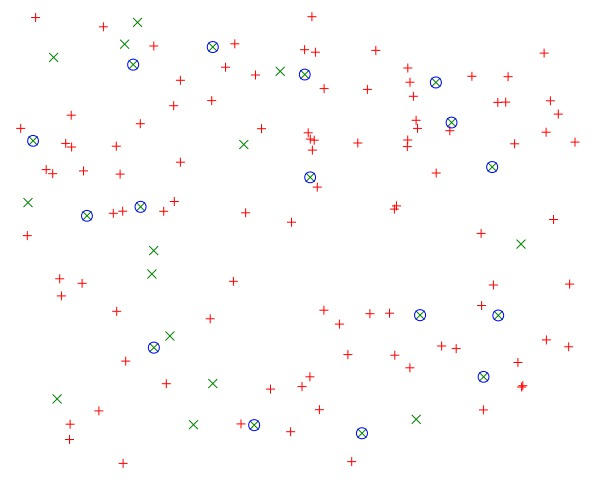
\includegraphics[scale=0.35]{Test_100_30_16_15}\caption{n = 100, m = 30, p = 16, l = 15}}\end{figure}}
\frame{\begin{figure}[h!]\centering{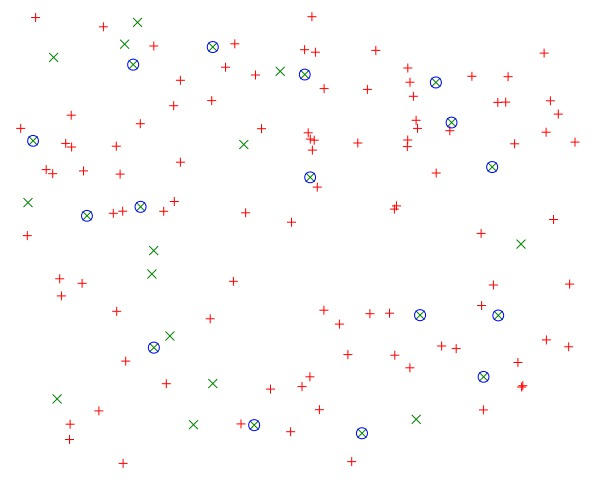
\includegraphics[scale=0.35]{Test_100_30_16_16}\caption{n = 100, m = 30, p = 16, l = 16}}\end{figure}}


\subsection{Background}
\begin{frame}[allowframebreaks]
  Richard Larson (1974) \cite{larson1974hypercube,larson1975approximating}
  proposes the Hypercube, and A-Hypercube models
  for a queuing approach for locating multiple facilities.

  James P. Jarvis (1985) \cite{jarvis1985approximating} incorporates
  location dependent service times characteristics for the A-Hypercube model,
  developing an approximation model for a spatially distributed queuing system
  under general service time assumptions.

  Berman et al. (1987) \cite{berman1987stochastic}
  formulate the Stochastic Queue p-Median problem (SQpM),
  and propose a heuristic approach for locating cooperative service facilities
  on a network.

  Goldberg et al. (1990) \cite{goldberg1990validating}
  propose a nonlinear integer programming model
  based on general service time approximation
  for spatially distributed queuing systems.

\end{frame}

\subsection{Hypercube queueing model}
\begin{frame}
Solution procedures for probabilistic models that use the hypercube model
with optimization procedures 
for server deployment can be found in the literature, for example
Larson (1979) \cite{larson1978structural}, 
Berman et al. (1985,1987) \cite{berman1985optimal,berman1987stochastic}, 
Saydam and Aytug (2003) \cite{saydam2003accurate}, 
Rajagopalan et al. (2008) \cite{rajagopalan2008multiperiod} and 
Iannoni et al. (2008a, 2008b) \cite{iannoni2008hypercube,iannoni2009optimization},
\end{frame}

%%% Solution methods %%%

%Emergency service systems: 
%The use of the hypercube queueing model in the solution of probabilistic location problems

\section{Hypercube queueing model}
\begin{frame}
Given a system configuration, 
the hypercube model is able to evaluate a variety of performance
measures relevant for decision-making, 
either region-wide or for each server or region.

These include 
server workloads, 
mean user response times, 
fraction of dispatches of each server to each region,
among others.
\end{frame}

\begin{frame}
There are some basic assumptions for the application of the hypercube model:
\begin{enumerate}
\item Geographical atoms and arrival processes
\item Servers and service processes
\item Server assignment and fixed-preference dispatching
\end{enumerate}
\end{frame}

\subsection{Calibration process of the mean service times}
\begin{frame}
In this emergency system, 
travel times may represent a considerable part of service times. 
It may be advisable to adjust the service times by means of a calibration process,
which can be performed using a simple iterative procedure.

The procedure consists of 
verifying if there are significant differences among 
the input mean service times and the output mean service times (computed by the hypercube model). 
In this case, 
the hypercube is solved using the computed mean service times as inputs, 
until the differences among input and output values are sufficiently small
\end{frame}

\begin{frame}{Probabilistic location models for planning ESSs}

Solution procedures for probabilistic models that use the hypercube model
Further studies combining the hypercube model with optimization procedures for server
deployment can be found in the literature; 
Larson (1979), 
Berman et al. (1985,1987), 
Saydam and Aytug (2003), 
Rajagopalan et al. (2008) and 
Iannoni et al. (2008a, 2008b).
\end{frame}

Conclusions

Conclusions are the last section people read in your paper, and therefore it’s what they leave remembering. You need to make sure they walk away thinking about your paper just the way you want them to.

Your conclusions needs to do three main things:

    Recap what you did. In about one paragraph recap what your research question was and how you tackled it.
    Highlight the big accomplishments. Spend another paragraph explaining the highlights of your results. These are the main results you want the reader to remember after they put down the paper, so ignore any small details.
    Conclude. Finally, finish off with a sentence or two that wraps up your paper. I find this can often be the hardest part to write. You want the paper to feel finished after they read these. One way to do this, is to try and tie your research to the “real world.” Can you somehow relate how your research is important outside of academia? Or, if your results leave you with a big question, finish with that. Put it out there for the reader to think about to.
    Optional Before you conclude, if you don’t have a future work section, put in a paragraph detailing the questions you think arise from the work and where you think researchers need to be looking next.

%Things to not do in your conclusion:

%   Introduce new information. The conclusion is for wrapping up everything you’ve done. It’s not a place to say “oh yeah, and we also got result y.” All results should be first presented and detailed in the result section. Think of the conclusion as a place to reflect on what you’ve already said earlier in the paper.
%   Directly re-quote anything you’ve already written. I’ve seen conclusions that are almost identical to the abstract or a collection of sentences from throughout the paper. As a reader, it makes me think the author was lazy and couldn’t be bothered to actually summarize their results for the paper. Take the time to write a proper conclusion so that the reader walks away with good thoughts about your work.
%   Write a conclusion longer than your introduction. A conclusion should be short, and to the point. You’ll rarely see them over 3 paragraphs, and three is often long. A lot of the time they are usually only one or two. Think about a conclusion as a chance to see how concisely you can summarize your entire research project. It’s your “30 second” research spiel.

\section{Future Work}
\begin{frame}{Future Work}
  \begin{itemize}
  \item Develop a simulator to evaluate the quality of the solutions
  \item Design and implement heuristic methods to solve larger instances
  \item Generate instances from real data
  \end{itemize}
\end{frame}


\subsection{Acknowledgements}
\begin{frame}{Acknowledgements}
\begin{itemize}
\item CONACYT (Graduate Fellowship)
\item CONACYT (grant 2011-1-166397)
\item UANL
\item FIME
\end{itemize}

\end{frame}

%%% References %%%
\begin{frame}[allowframebreaks]
  %\setbeamertemplate{bibliography item}{\insertbiblabel}
  \frametitle{References}
  {\scriptsize
    \bibliographystyle{abbrv}
    \bibliography{references}
  }
\end{frame}
\end{document}
